\documentclass[psamsfonts]{amsart}
\usepackage[utf8]{inputenc}
\usepackage{amsfonts}
\usepackage{hyperref}
\usepackage{amsmath}
\usepackage{xcolor}
\usepackage{amsthm}
\usepackage{pdflscape}
\usepackage{pgfplots}
\usepackage{mathrsfs}
\usepackage{setspace}
\usepackage[margin=1in]{geometry}
\usepackage{subcaption}

% \setlength{\abovedisplayskip}{15pt}
% \setlength{\belowdisplayskip}{15pt}
% \setlength{\abovedisplayshortskip}{15pt}
% \setlength{\belowdisplayshortskip}{15pt}

\newcommand{\rme}{\mathrm{e}}  
\newcommand{\rmd}{\mathrm{d}}       

\newcommand{\C}{\mathbb{C}}
\newcommand{\N}{\mathbb{N}}
\newcommand{\Q}{\mathbb{Q}}
\newcommand{\A}{\mathbb{A}}
\newcommand{\R}{\mathbb{R}}
\newcommand{\Ell}{\mathscr{L}}
\newcommand{\Z}{\mathbb{Z}}
\newcommand{\E}{\mathbb{E}}
\newcommand{\K}{\mathbb{K}}
\newcommand{\F}{\mathbb{F}}
\newcommand{\PP}{\mathbb{P}}

% \setstretch{1.0}

\newtheorem{thm}{Theorem}[section]
\newtheorem{cor}[thm]{Corollary}
\newtheorem{prop}[thm]{Proposition}
\newtheorem{lem}[thm]{Lemma}
\newtheorem{conj}[thm]{Conjecture}
\newtheorem{quest}[thm]{Question}
\newtheorem{claim}[thm]{Claim}
\newtheorem{ppty}[thm]{Property}

\theoremstyle{definition}
\newtheorem{defn}[thm]{Definition}
\newtheorem{defns}[thm]{Definitions}
\newtheorem{con}[thm]{Construction}
\newtheorem{exmp}[thm]{Example}
\newtheorem{exmps}[thm]{Examples}
\newtheorem{notn}[thm]{Notation}
\newtheorem{notns}[thm]{Notations}
\newtheorem{addm}[thm]{Addendum}
\newtheorem{exer}[thm]{Exercise}
\newtheorem{limit}[thm]{Limitation}


\theoremstyle{remark}
\newtheorem{rem}[thm]{Remark}
\newtheorem{rems}[thm]{Remarks}
\newtheorem{warn}[thm]{Warning}
\newtheorem{sch}[thm]{Scholium}

\makeatletter
\let\c@equation\c@thm
\makeatother
\numberwithin{equation}{section}

\bibliographystyle{plain}

%--------Meta Data: Fill in your info------
\title[Identifying a phase transition between emergent dynamics of stochastic CTLNs]{Identifying a phase transition between emergent dynamics in stochastic Combinatorial Linear-Threshold Networks}
\author{Eric Han, Caitlin Lienkaemper}

\begin{document}

\begin{abstract}
Within the field of computational neuroscience, there has been a recent model of interest known as the Combinatorial Linear-Threshold Network model (CTLN).The CTLN model is a simplified mathematical model that focuses on the intricate connectivity between neurons as the key factor affecting the resulting dynamics of the network. Emergent dynamics are nonlinear and complex, demonstrating coalescence to fixed points as well as possession of chaotic attractors. Utilizing the vocabulary of combinatorial graph theory and oriented matroids to represent neural networks, previous literature has focused on the dynamical regimes that any particular architecture can support. Within this paper, we focus primarily on a stochastic approach that characterizes graphs based on two key parameters, and then analyze the dynamics of graphs with specific parametrized characteristics rather than focusing on any specific structural pattern. We identify a phase transition between the two unique dynamical regimes exhibited by these networks.
\\\\
% \noindent \textbf{Keywords.} Derivative, Differential calculus, Differentiation, Taylor's theorem, Taylor's formula, Taylor's series, Taylor's polynomial, Power function, Binomial theorem, Smooth function, Newton's interpolation formula, Finite difference, Q-derivative, Jackson derivative, Q-calculus, Quantum calculus, Q-difference, Quantum algebra\\\\
% \noindent MA 562, Methods of Applied Math 2 \\
% \noindent Professor Gabriel Ocker \\
% \noindent Final Project\\
\noindent \textbf{Email:} ehan08@bu.edu, Caitlin email tba\\
% \noindent \textbf{Date:} April 26, 2024
\end{abstract}

\maketitle
\tableofcontents
\newpage

\section{Introduction}

The dynamics of threshold-linear networks are governed by the following ODE:
\[
    \frac{dx_i}{dt} = -x_i + \left[ \sum^{n}_{j=1} W_{ij} x_j + \theta \right]_+ \mbox{, i = 1, 2,\dots, n},
\]
where $n$ is the number of neurons. $x_i$ represents the firing rate of the $i$-th neuron and $\theta>0$ is a constant external input. $W_{ij}$ is an $n\times n$ matrix that describes the connective strength between neurons $i,j$. The threshold non-linearity as described by $[\cdot]_+ := \max\{0,\cdot\}$ produces nonlinear dynamics within the network. CTLNs are a special case of the TLN model where we restrict connection strengths in $W_{ij}$. The network exhibits a variety of complex dynamical regimes, including multistable behavior, and can also possess limit cycles and multiple chaotic attractors.

By electing to use $W_{ij}$ as a connectivity matrix for a directed graph $G$, we are able to tightly link specific dynamical behavior to graph structure.
\\

In existing literature, there has been a great deal of emphasis on specific small-scale network structures. In particular, there is a focus on the emergence of fixed-point support structures. An important conjecture attempts to classify all fixed point supports as sets of all-connected, target-free vertices. In our paper, instead of observing explicit structural patterns present on networks, we classify networks probabilistically and observe the average dynamics manifested by these networks.
\\

In order to analyze CTLNs as a stochastic system, we must be able to parametrize characteristics of the CTLN that affect the dynamics manifested. The easiest and most intuitive way to do this is to parametrize edge connection probability as well as the symmetry of the graph. That is, we assign values to how ``bidirectional'' our network is. A completely symmetric network would be an undirected graph, while a completely asymmetric graph would only contain unidirectional edges. We then generate random graphs with these parameters and attempt to discern the average dynamics of a size $n$ system with specific combinations of edge connection probability and symmetry.

Through numerical simulation, we have generated heatmaps of averaged network dynamics that showcase general patterns for size-$n$ networks across the full spectrum of edge-connection probabilities $p$ and degrees of symmetry $q$. Utilizing these heatmaps, we see a distinct zone of phase transition where dynamics go from coalescing to a fixed point to exhibiting strongly chaotic behavior. Additionally, it should be noted that chaotic behavior persists for longer for large $n$ graphs.\\

\section{Random Graphs} % (fold)
\label{sec:random_graphs}

% section random_graphs (end)
Formally, $G(N,p,q)$ is a \textbf{random graph} generated using the Erd{\"o}s-Renyi random graph model with an additional symmetry parameter $q$.

\begin{defn}[Symmetry]
  Let $i,j$ be any two vertices with an edge between them in a directed graph. $i$ and $j$ are considered \textit{symmetric} if there exists a bidirectional edge between them. A graph is considered fully symmetric if every edge in the graph is a bidirectional edge; or if there exist no edges in the graph.
\end{defn}
$N$ denotes the number of vertices that the graph has, which we will refer to as graph size, and $0\leq p\leq 1$ denotes the edge generation probability. That is, begin with an empty graph with a set of vertices $\{n\}$ such that $|\{n\}|=N$. We conduct $\binom{n}{2}$ Bernoulli experiments generating edges independently. The probability of the generation of a bidirectional edge is given by $pq$, generation of a forward edge is given by $p\left(\frac{1-q}{2}\right)$, generation of a backward edge is given by $p\left(\frac{1-q}{2} \right)$, and no edge generation is given by $1-p$.\footnote{https://www.math.cmu.edu/~af1p/BOOK.pdf}

From previous literature, for any fixed point $x\in\R^n$, the support of a fixed point is given by 
\[
  \sigma = \{i\in\{1,\ldots,n\} : x_i>0\}
.\] 
It has been shown that target-free cliques are fixed-point supports. 
\begin{defn}[Clique]
  Let $G(N)$ be a directed graph of size $N$. Then, any set of all-connected vertices forms a clique of size $k$, $\varphi_k$. Let $\varphi_k = \{v_i:i\in\{1,\ldots,n\}\}$ for $n < N$. If $\varphi_k$ cannot be made larger by including another vertex $v_j$, then $\varphi_k$ is \textbf{maximal}.
\end{defn}
As a consequence, for a graph $G(N)$, a clique of size $N$ is always maximal.
Additionally, we utilize the following conjecture:
\begin{conj}
  \label{conj:fp_supp}
  Let $W_{ij}(G)$ denote a CTLN on a graph $G$ and let $\sigma\subseteq G$. Then, $\sigma$ is the support of a stable fixed point if and only if $\sigma$ is a target-free clique.
\end{conj}

We begin with a pair of theorems that allow us to determine the expected number of target-free cliques of size $k$, $\sigma_k$, in a graph $G$.
\begin{thm}
  The expected number of $k$-sized cliques for a graph $G(N,p,q)$ is given by
  \begin{equation}
    \label{eq:exp_max_directed}
    \E[\varphi_k] = \binom{N}{k}(pq)^{\binom{k}{2}}
     % \left(1-p\left(\frac{1-q}{2}\right)\right)^{N-k}
     .
  \end{equation}
\end{thm}

\begin{thm}
  The probability of a $k$-sized clique being target-free is given by
  \begin{equation}
    \label{eq:p_targetfree_directed}
    \PP(\varphi_k \mbox{ is target-free }|\varphi_k \mbox{ exists}) = \left[ 1- \left(pq + p   \left(\frac{1-q}{2} \right) \right)^k \right]^{N-k}.
  \end{equation}
\end{thm}

Due to the independence of edge generation under the Erd{\"o}s-Renyi random graph model, we are able to directly compute the expected number of target-free cliques of size $k$,
\begin{align}
  \label{eq:exp_tf_cliques}
  \E[\mbox{target-free } k\mbox{-cliques}] &= \E[\sigma_k] \cdot \PP(\sigma_k \mbox{ is target-free }|\sigma_k \mbox{ exists})
  \\
  & = \binom{N}{k}(pq)^{\binom{k}{2}} \left[ 1- \left(pq + p   \left(\frac{1-q}{2} \right) \right)^k \right]^{N-k} \notag
\end{align}

Utilizing conjecture $\ref{conj:fp_supp}$, this gives us the expected number of $k$-sized fixed point supports for any graph $G(N,p,q)$. Importantly, this allows us to observe the formation of maximal cliques over the entire parameter space $p,q$ as we take the large $N$ limit of $G(N,p,q)$. However, we are now faced with a new problem. We have naively suggested that $k$ be some arbitrary parameter that should implicitly grow with graph size. To remedy this issue, we define
\[
  k = \alpha N
\]
where $0\leq\alpha\leq1$. As such, equation \ref{eq:exp_tf_cliques} becomes
\begin{equation}
  \label{eq:exp_tf_w_a}
  h(N,p,q,\alpha) = \binom{N}{\alpha N}(pq)^{\binom{\alpha N}{2}} \left[ 1- \left(pq + p   \left(\frac{1-q}{2} \right) \right)^{\alpha N} \right]^{N-\alpha N}.
\end{equation}
We can then integrate this over $[0,1]$ against $\alpha$ to observe the effects of $\alpha$ across the entire $p,q$-space.\footnote{wording}

This is very difficult - perhaps we use a gamma function representation?
\[
  \frac{\Gamma(N+1)}{\Gamma(k+1)\Gamma(N-k+1)} (pq)^{\frac{k(k-1)}{2}} \left[ 1- \left(pq + \frac{p(1-q)}{2} \right)^k \right]^{N-k}
\]
% \begin{align*}
%   \label{eq:integral}
%   &\int_{0}^{1} \binom{N}{\alpha N}(pq)^{\binom{\alpha N}{2}} \left[ 1- \left(pq + p   \left(\frac{1-q}{2} \right) \right)^{\alpha N} \right]^{N-\alpha N} d\alpha.
% \end{align*}\\
\\

In order to make equation \ref{eq:exp_tf_w_a} more numerically and analytically tractable, we expand the binomial coefficients and then use Stirling's approximation for factorials. 

Stirling's approximation for factorials is given as
\[
  n! \sim \sqrt{2\pi n} \left(\frac{n}{e}\right)^n.
\]
This approximation is extremely accurate for large values of $N$. The ratio between the two quantities tends to $1$ as $N$ tends to $\infty$.

So, we arrive at
\[
  h(N,p,q,\alpha) = \frac{\sqrt{2\pi N} \left(\frac{N}{e}\right)^N}{\sqrt{2\pi\alpha N} \left(\frac{\alpha N}{e}\right)^{\alpha N} \sqrt{2\pi N(1-\alpha)} \left(\frac{N(1-\alpha)}{e}\right)^{N(1-\alpha)}}
  \left(pq\right)^{\frac{\alpha N (\alpha N - 1)}{2}}
  \left[1-\left(p\left(\frac{1-q}{2}\right)+pq\right)^{\alpha N}\right]^{N(1-\alpha)}.
\]
As we take the large $N$ limit of this quantity, 

\section{Proofs} % (fold)
\label{sec:proofs}

% section proofs (end)

\section{Numerics} % (fold)
\label{sec:numerics}
Detailed below are the numerical methods used and their resulting simulations. These are the grounds that spurred the main goal of the paper.

To generate dynamics for individual graphs, we used a standard iterative method for numerically solving PDEs.
\begin{figure}[h]
     \centering
     \begin{subfigure}{0.45\textwidth}
         \centering
         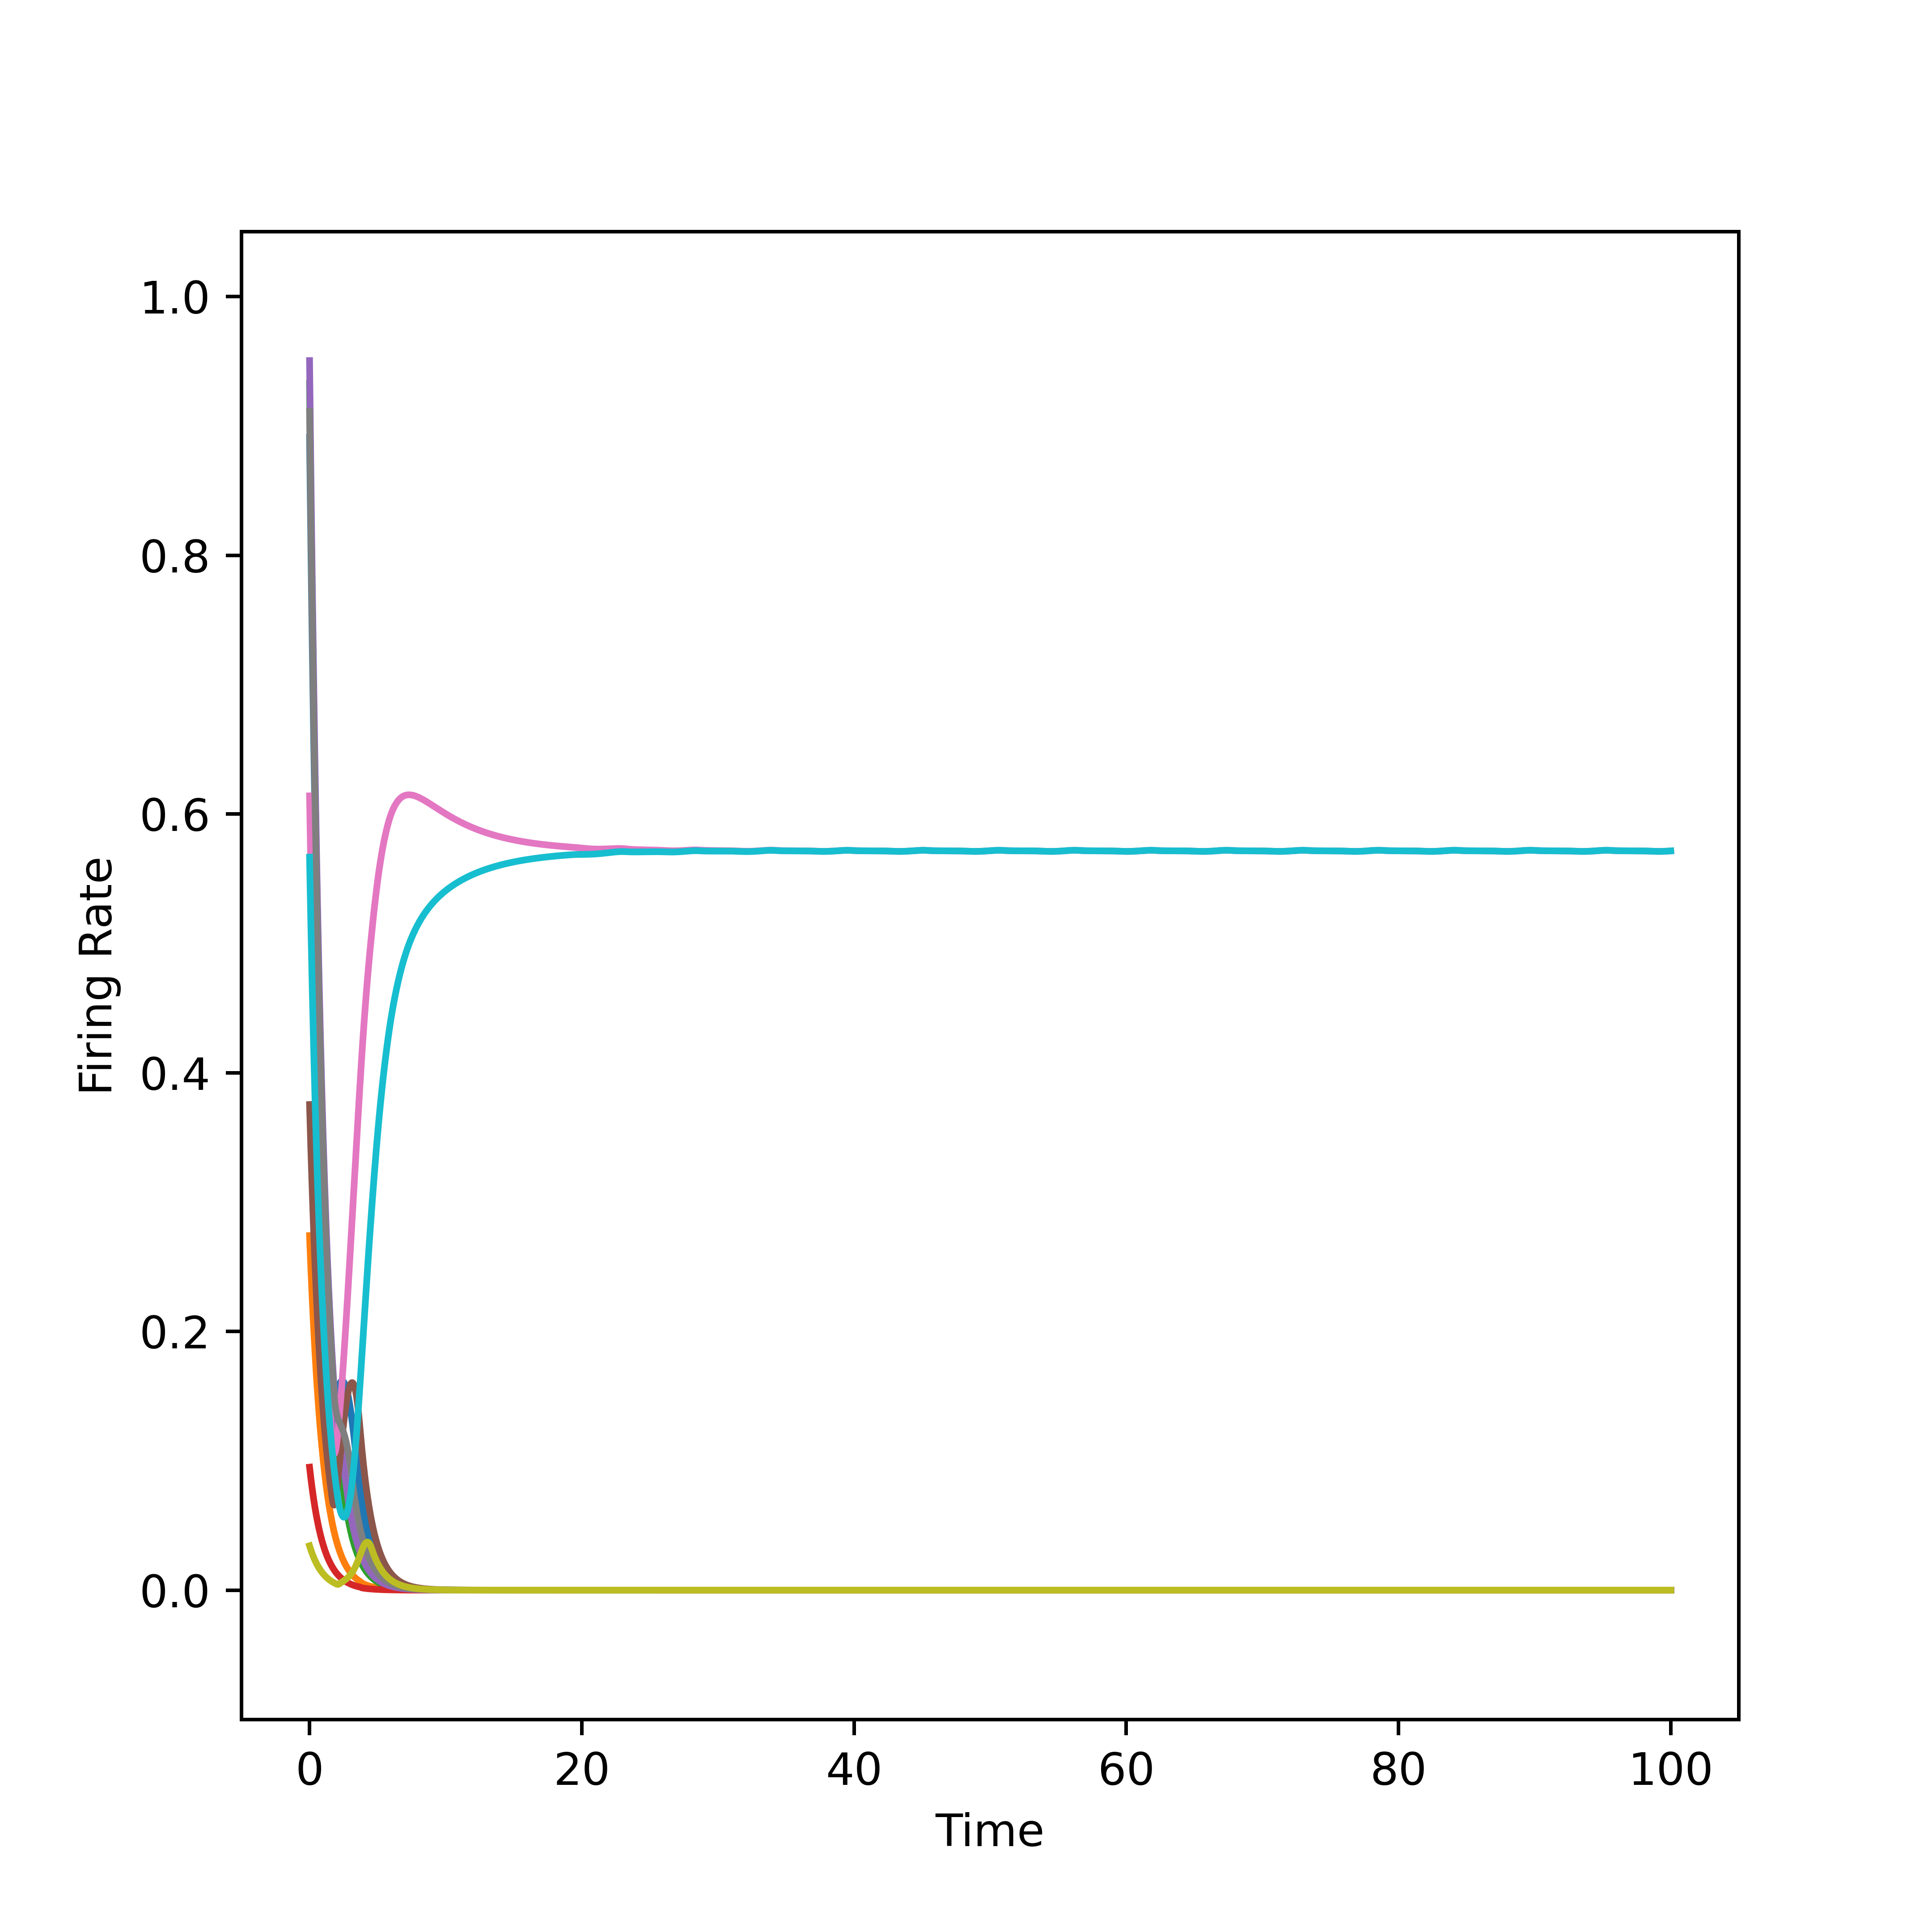
\includegraphics[scale = 0.4]{./Figures/Matrix Size 10 Symmetry 0.100 0.6 0.1 12.png}
         \label{fig:1a}
     \end{subfigure}
     \begin{subfigure}{0.45\textwidth}
         \centering
         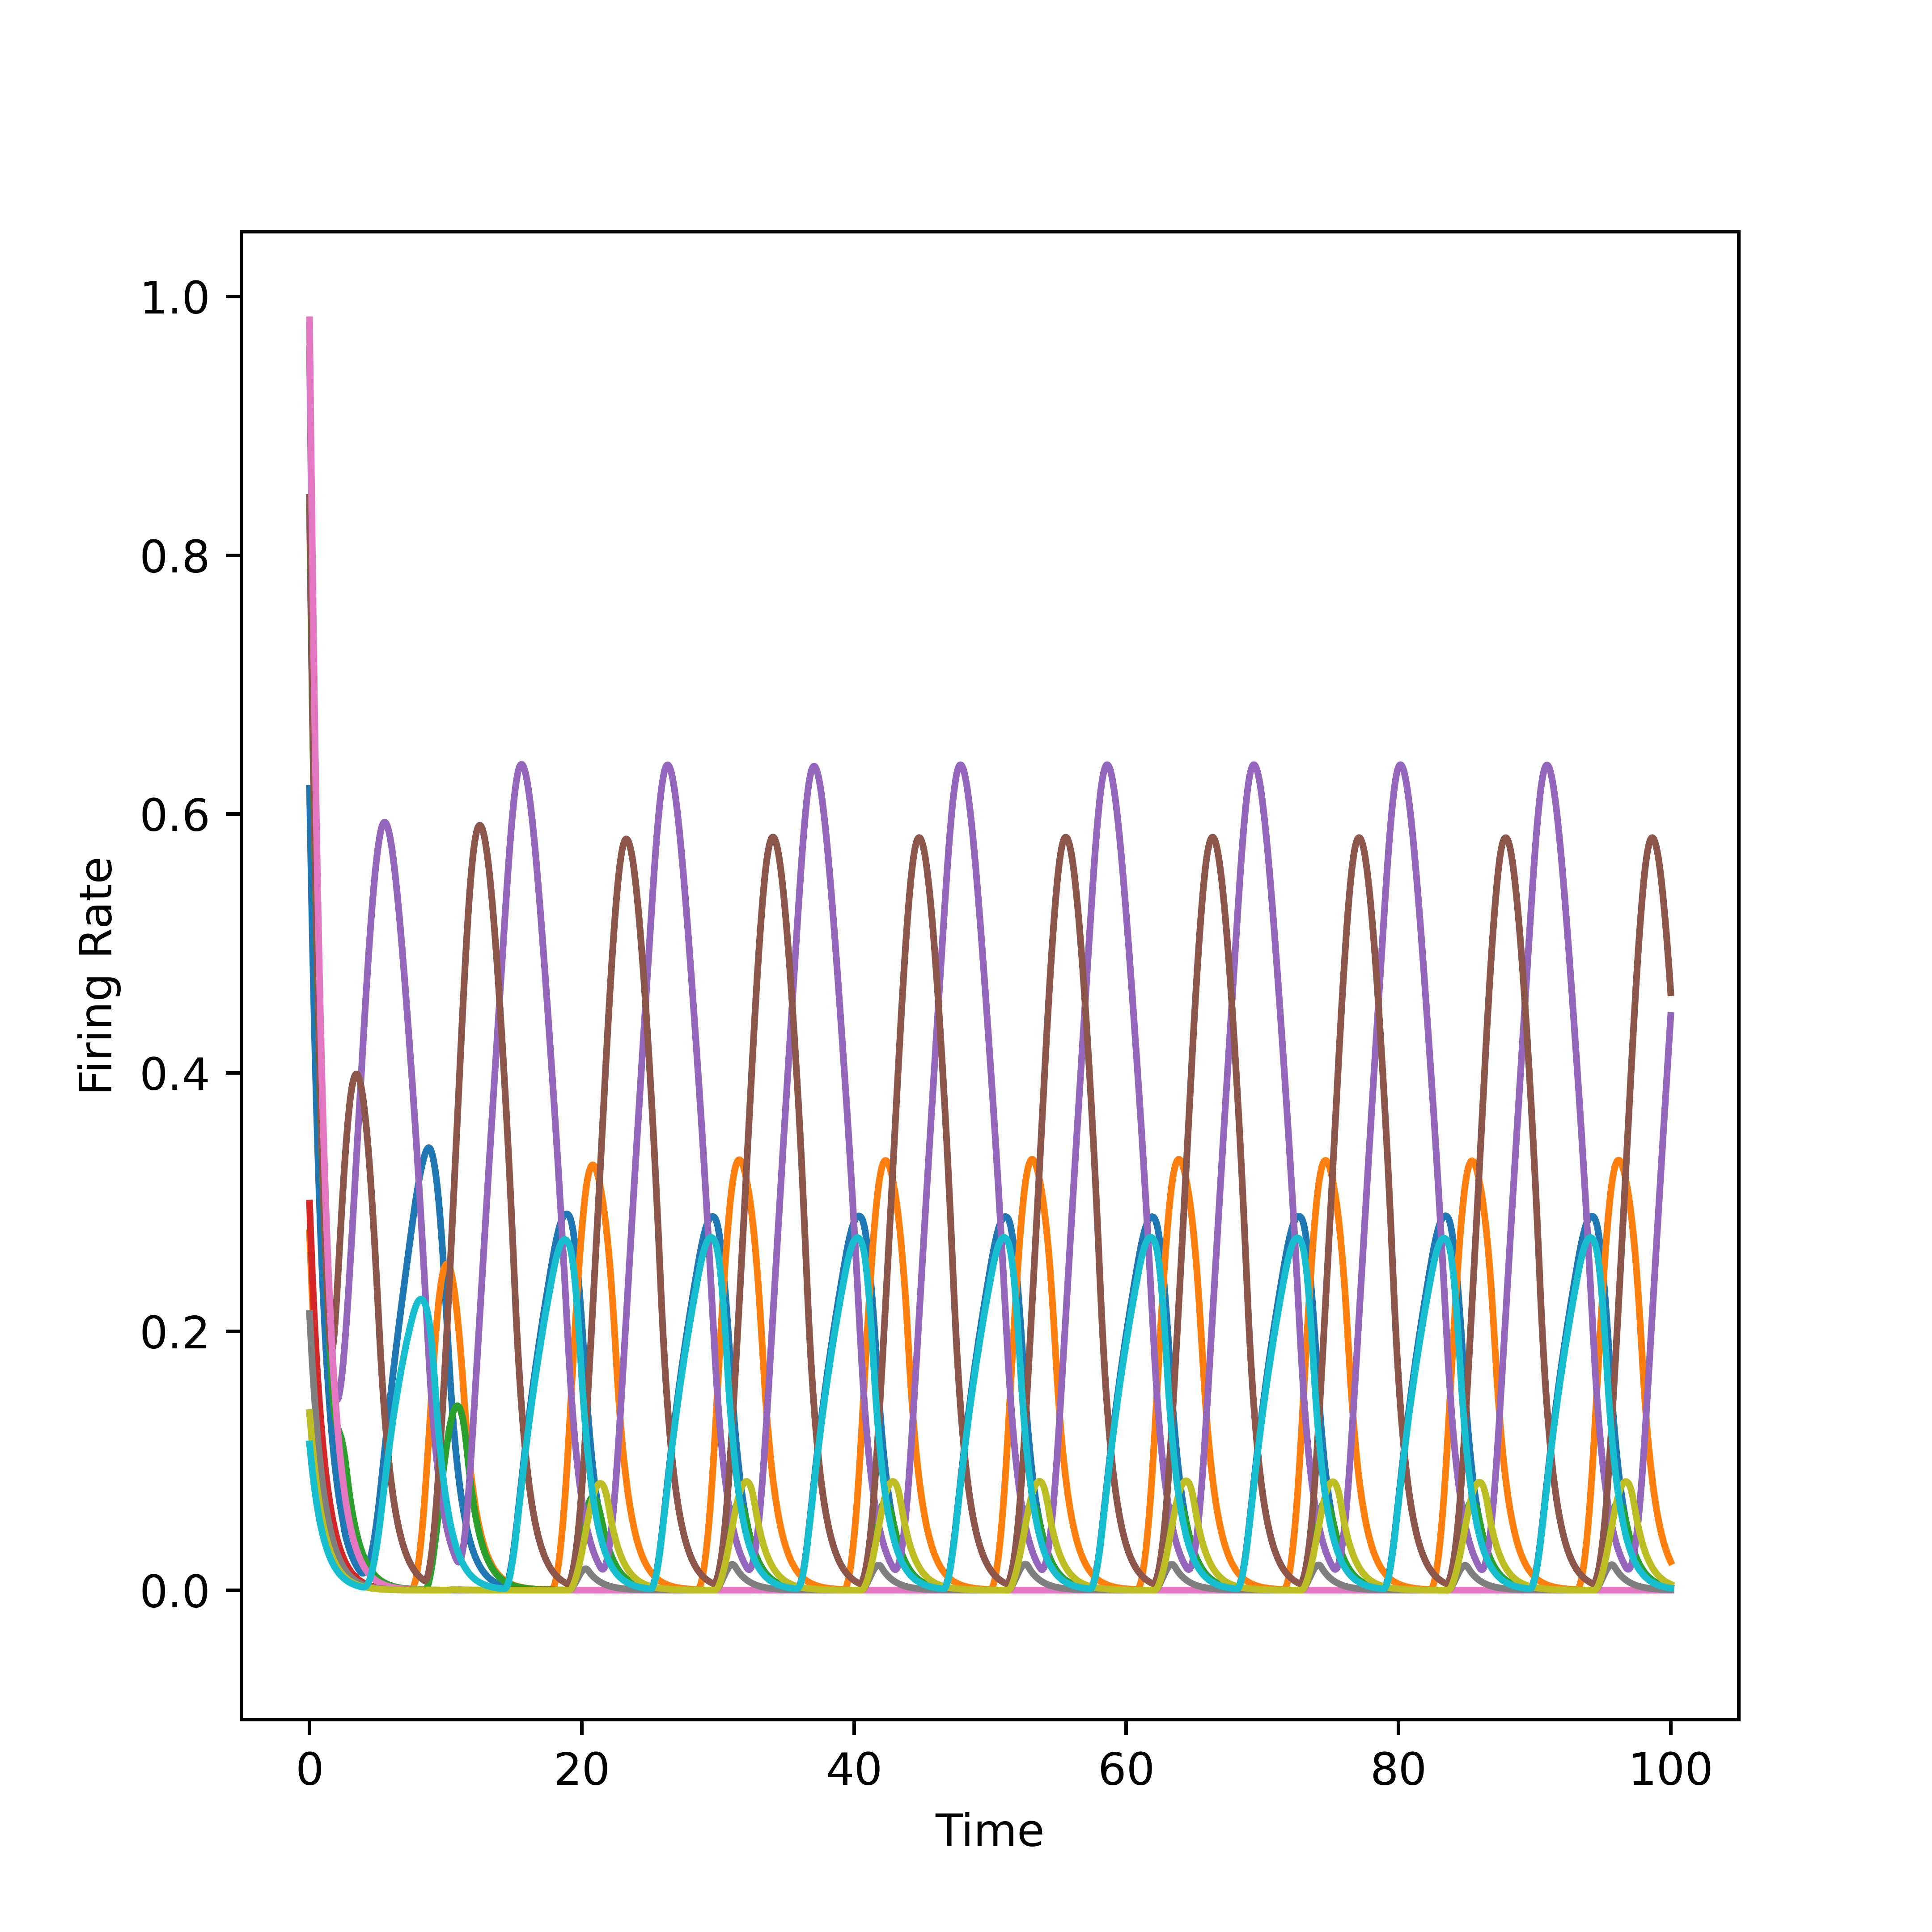
\includegraphics[scale = 0.4]{./Figures/Matrix Size 10 Symmetry 0.100 0.6 0.1 13.png}
         \label{fig:1b}
     \end{subfigure}
     \caption{Two 15-networks demonstrating different behavior despite having the same parameters. $N=15, p=0.6, q=0.1$. This highlights the variance in network dynamics, even in small networks. We conjecture that as network size is increased, outliers are less likely to occur, but coalescence to a steady state is much slower.}
     \label{fig:1}
\end{figure}

Accurate simulation of network dynamics means that we may average the behavior of randomly-generated networks across the entire spectrum of symmetry-edge connection values. To do this, we simply simulate the dynamics of networks with specific parameters multiple times in order to generate heatmaps that indicate how likely a specific pair of parameters is to result in a fixed point. We detect fixed points by numerically computing the derivatives at the final point in time.

\begin{figure}[h]
     \centering
     \begin{subfigure}{0.45\textwidth}
         \centering
         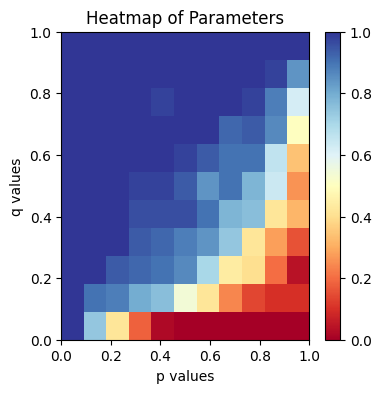
\includegraphics[width=\linewidth]{./Figures/size 30 heatmap 2.png}
         \label{fig:1a}
     \end{subfigure}
     \begin{subfigure}{0.45\textwidth}
         \centering
         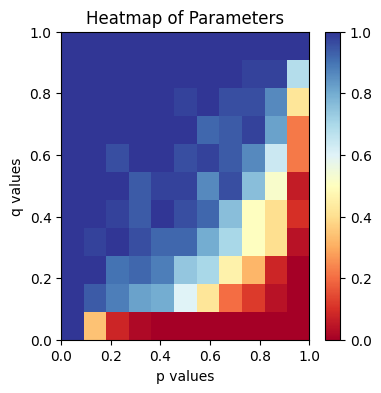
\includegraphics[width=\linewidth]{./Figures/size 50 heatmap.png}
         \label{fig:1b}
     \end{subfigure}
     \caption{Averaged heatmaps for a 30-network (left) and a 50-network (right). Heatmaps were averaged over 7 trials. Red regions are more likely to coalesce to a limit cycles and blue regions are more likely to coalesce to a fixed point. One can clearly see a distinct zone of phase transition where firing rate trajectories ``shift'' to the other steady state. As network size grows, the phase transition becomes more prominent and pairs of parameters become more ``patterned''.}
     \label{fig:1}
\end{figure}




% section numerics (end)

\end{document}